\section{Utility and Risk Awearness}
\label{sec:utilityAnRisk}

Classical HTN planners have several advantages over classical planners, but they lack any concept of utility. Classical HTN planners are satisfied when a solution is found, but in the real world, this is rarely sufficient. In the real world, we are typically interested in finding an optimal solution in some sense. For instance, we may only be interested in solutions that are safe, fast, or inexpensive. In this section, we will provide an overview of the notion of utility and how it can be utilized to guide the planning process.

\subsection{Utility}
The core concept of utility revolves around modeling the outcomes of an action or situation based on a set of criteria or metrics, which allows us to rank actions or outcomes and choose the most preferable option. Mathematically, utility can be represented via a set of binary relations over a set of actions or situations $\mathbf{\Delta}$ \cite{fishburn1968utility}.

\begin{Tdef}[Preference-indifference relation $\preceq$]
    The preference-indifference relation $\preceq$ is a binary relation over a set of actions/situations $\mathbf{\Delta}$ that satisfies the following:
    $$\forall \delta_1, \delta_2 \in \Delta : \delta_1 \preceq \delta_2 \vee \delta_1 \npreceq \delta_2$$
    $\delta_1 \preceq \delta_2$ means that $\delta_1$ is not preferred to $\delta_2$.
\end{Tdef}

\begin{Tdef}[Strict preference relation $\prec$]
    The strict preference relation $\prec$ is a binary relation over a set of actions/situations $\mathbf{\Delta}$ that satisfies the following:
    $$\forall \delta_1, \delta_2 \in \Delta : \delta_1 \prec \delta_2 \Longleftrightarrow \delta_1 \preceq \delta_2 \wedge \delta_2 \npreceq \delta_1$$
    $\delta_1 \prec \delta_2$ means that $\delta_2$ is preferred to $\delta_1$.
\end{Tdef}


\begin{Tdef}[Indifference relation $\sim$]
    The indifference relation $\sim$ is a binary relation over a set of actions/situations $\mathbf{\Delta}$ that satisfies the following:
    $$\forall \delta_1, \delta_2 \in \Delta : \delta_1 \sim \delta_2 \Longleftrightarrow \delta_1 \preceq \delta_2 \wedge \delta_2 \preceq \delta_1$$
    $\delta_1 \sim \delta_2$ means that $\delta_1$ is indifferent to $\delta_2$.
\end{Tdef}

The previous binary relations form an invaluable framework that enables us to rank solutions given that we have a model that can map any action/situation to a numeric value (utility). It is essential to recognize that utility and value do not constitute the same concept. For example, in the context of commuting to work, one can use the train or a taxi. The train would cost two dollars, whereas the taxi would cost twenty. These values do not take into consideration factors such as comfort, speed, or emissions. Concrete values such as cost and time are objective, whereas utility is quite subjective. An agent with an emphasis on comfort would give the train a lower utility score, while an agent with an emphasis on reducing emissions would give the train a higher utility score.


\subsection{Utility based HTN planning}
One way of utilizing utility to guide an HTN planner is to assign each operator a utility score, but this is insufficient. HTN structures are intrinsically hierarchical, and the utility of a task is not necessarily identical to the utility of its subtasks. A significantly better approach is to assign a utility score to each operator, method, and compound task. The utility of a task is then the sum of its own utility and the utility of its most preferred subtask. It is essential to bear in mind that utility is extremely dynamic, and thus the planner needs to be able to recalculate the utility of each task as the planning process progresses or whenever the state of the environment changes.

\begin{figure}[H]
    \centering
    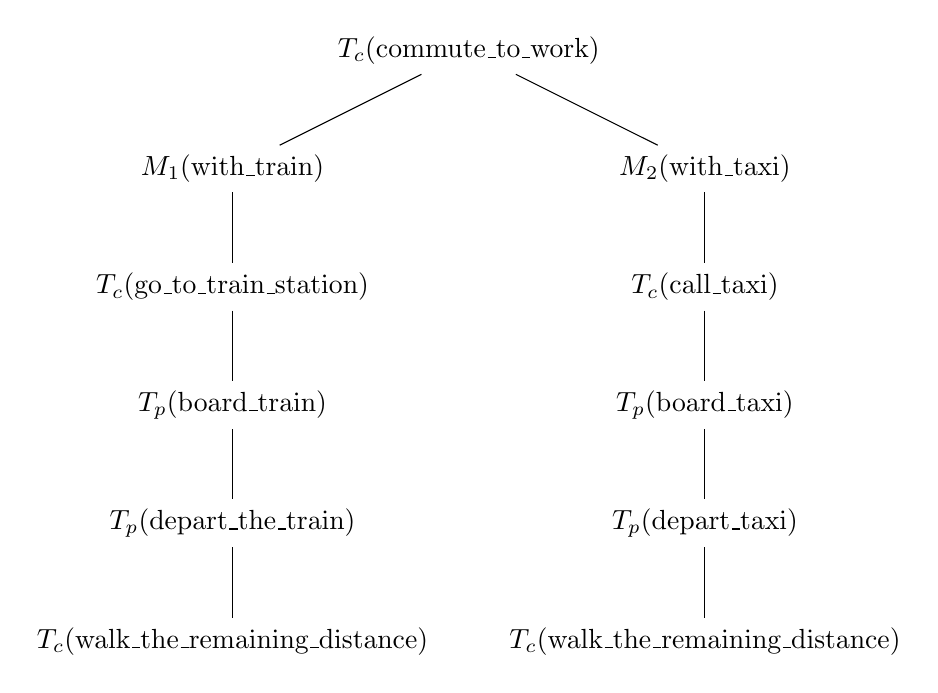
\begin{tikzpicture}
        \node {$T_c$(commute\_to\_work)} [sibling distance = 6cm]
            child { 
                node{$M_1$(with\_train)} 
                child{ 
                        node{$T_c$(go\_to\_train\_station)}
                        child {
                            node{$T_p$(board\_train)}
                            child {
                                node{$T_p$(depart\_the\_train)}
                                child{
                                    node{$T_c$(walk\_the\_remaining\_distance)}
                                }
                            }
                        }
                    }
                }
            child {
                node{$M_2$(with\_taxi)}
                child{ 
                        node{$T_c$(call\_taxi)}
                        child {
                            node{$T_p$(board\_taxi)}
                            child {
                                node{$T_p$(depart\_taxi)}
                                child{
                                    node{$T_c$(walk\_the\_remaining\_distance)}
                                }
                            }
                        }
                    }
                };
    \end{tikzpicture}
    \caption{A simple HTN task network for commuting to work.}
    \label{fig:commute_to_work}
\end{figure}
Figure ~\ref{fig:commute_to_work} shows a simple HTN task network for commuting to work. This example will help us to illustrate the necessity of having a utility score for each HTN construct. If we exclusively assign utility values to the operators, there will be no way to express whether an agent prefers or dislikes using the train for example. The compound task \qq{walk\_the\_remaining\_distance} can be reached via two distinct paths, and it would be illogical to assign it the same utility in both scenarios. The compound task \qq{commute\_to\_work} itself could have an inherently low utility value if the agent prefers to work from home.

We will refrain from providing a concrete algorithm for integrating utility into HTN planning since it is highly dependent on the search strategies implemented by the planner and because it has already been done in \cite{alnazer2019htn} \cite{georgievski2014utility} \cite{alnazer2022risk}. However, we will go over our own implementation in detail later on.

\subsection{Expected utility}
Basic utility is an effective tool for comparing solutions and ensuring that the agent always chooses the solution with the most preferable outcome. However, basic utility assumes that the world is deterministic and each action has only one outcome, which has a significant impact on its applicability in the real world, where uncertainty is a fundamental challenge.
To illustrate the limitations of basic utility, consider the following scenario shown in Figure~\ref{fig:expected_utility} in which an agent is offered the choice between two actions, $\delta_1$ and $\delta_2$. There are two possible outcomes for action $\delta_1$: the agent will receive three dollars 40\% of the time, and nothing the remaining 60\% of the time. Action $\delta_2$ also has also two possible outcomes: 10\% of the time, the agent will receive seven dollars, and 90\% of the time, it will receive nothing.

\begin{figure}[H]
    \centering
    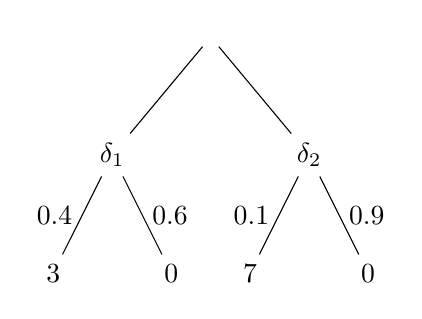
\begin{tikzpicture}
        \node {} [sibling distance = 2.5cm]
            child{
                node{$\delta_1$}[sibling distance = 1.5cm]
                child{node{3} edge from parent node [left] {0.4}}
                child{node{0} edge from parent node [right] {0.6}}
            }
            child{
                node{$\delta_2$}[sibling distance = 1.5cm]
                child{node{7} edge from parent node [left] {0.1}}
                child{node{0} edge from parent node [right] {0.9}}
            };
        \end{tikzpicture}
        \caption{A simple example of hypothetical game.}
        \label{fig:expected_utility}
\end{figure}

If the agent is acting solely on the basis of basic utility, it will always choose action $\delta_2$, since its utility value is greater, whereas a rational agent will virtually always choose action $\delta_1$ because it has a greater expected value:
$$ \mathbbm{E}(\delta_2) = 0.1 \times 7 + 0.9 \times 0  < \mathbbm{E}(\delta_1) = 0.4 \times 3 + 0.6 \times 0 $$

In the previous example, we assumed that the agent based its decision on the expected value, which can lead us to the wrong conclusion that expected value can be used to represent expected utility. However, it was clear from the early stages of research that rational agents do not always act on the basis of expected value. As previously discussed, value is an objective concept, whereas utility is far more subjective and can be influenced by an agent's preferences, needs, and risk tolerance. Expected value fails to capture the subjective nature of utility, and thus it is not a suitable tool for representing expected utility. To further illustrate this point, we need to introduce the \textbf{St. Petersburg paradox}\footnote{\url{https://en.wikipedia.org/wiki/St._Petersburg_paradox}}, which demonstrates how an agent whose only criteria for decision-making is expected value would propose a course of action that no rational agent would ever consider:

\begin{quotation}
    A hypothetical casino in St. Petersburg offers the following game to a single player:
    After paying a fixed entrance fee, a fair coin is tossed until the first head appears, which ends the game. When the game ends, the player wins $2^n$, where $n$ is the round where the first head appeared.
\end{quotation}

Now the question is \textit{how much would a rational agent be willing to pay as an entrance fee to play this game?}

An agent using the expected value would be willing to pay an entrance fee up to the game's expected value which is infinite:
$$  \mathbbm{E} = \frac{1}{2} \cdot 2 + \frac{1}{4} \cdot 4 + \frac{1}{8} \cdot 8 + \frac{1}{16} \cdot 16 + \dots = \infty$$

which contradicts the fact that no rational agent would be willing to pay an arbitrary large entrance fee to play this game. A better approach would be to define a utility function $\mathfrak{u}$ that reflects the agent's preferences. We can use $\mathfrak{u}$ to define the expected utility of an action $\delta$ over the probability distribution $\mathbbm{P}$ of all its possible outcomes $\Omega$.

\begin{Tdef}[Expected Utility]
    The expected utility of an action $\delta$ is the weighted sum of all possible outcomes of $\delta$:
    $$\mathbbm{E}(\delta) = \sum_{\omega} \mathbbm{P}(\omega) \cdot \mathfrak{u}(\omega)$$
\end{Tdef}

Using expected utility, we can extend our prefrence relations:
\vspace{-0.5em}
\begin{subequations}
    \begin{align*}
    \forall \delta_1, \delta_2 \in \Delta: \quad& \\
    & \delta_1 \preceq \delta_2 \Longleftrightarrow \mathbbm{E}(\delta_1) \leq \mathbbm{E}(\delta_2) \\
    & \delta_1 \prec \delta_2 \Longleftrightarrow \mathbbm{E}(\delta_1) < \mathbbm{E}(\delta_2) \\
    & \delta_1 \sim \delta_2 \Longleftrightarrow \mathbbm{E}(\delta_1) = \mathbbm{E}(\delta_2) \\
    \end{align*}
\end{subequations}

\subsection{Risk attitude}
As mentioned earlier, the utility function is a highly subjective model of the world that reflects the agent's preferences, most notably its risk tolerance. In this section, we provide a short overview of the standard risk attitude models and how the risk attitude can guide the behavior of an agent.

Sometimes rational agents are inclined to change behavior when the stacks are too high. For example, let us consider the following game, where a player has a 60\% chance of winning 100 dollars and a 40\% chance of losing 1 dollar. Some players would simply refuse to play the game because losing one dollar is too much of a risk. Some players would be willing to play the game, but they might also refuse to play if the stakes were higher. In other words, the risk attitude can be defined as the change in utility based on the ratio of potential wins to potential losses.

It is difficult to quantitatively model risk, and different fields have attempted to do so using different theories; since we cannot cover all of them here, we will explore the topic from the agent's viewpoint.

Maximizing gains or minimizing losses would be the primary goal of a naive agent. Such an agent would have an indifferent attitude toward risk (\textit{Risk neutral}). This type of agent will always choose a course of action that maximizes/minimizes its gains/losses, regardless of the risk involved.

\begin{figure}[H]
    \centering
    \begin{minipage}{.5\textwidth}
      \centering
      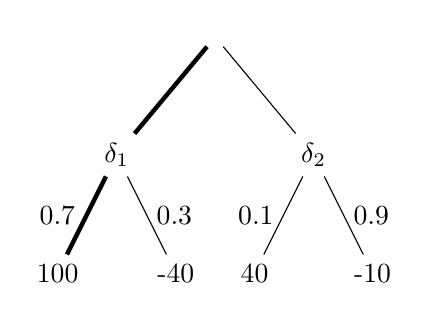
\begin{tikzpicture}
        \node (a){} [sibling distance = 2.5cm]
            child{
                node(b){$\delta_1$}[sibling distance = 1.5cm] 
                child{node(c){100} edge from parent[ultra thick] node [left,black] {0.7}}
                child{node(d){-40} edge from parent[solid, thin] node [right] {0.3}}
                edge from parent[ultra thick] 
            }
            child{
                node(e){$\delta_2$}[sibling distance = 1.5cm]
                child{node(f){40} edge from parent node [left] {0.1}}
                child{node(g){-10} edge from parent node [right] {0.9}}
            };
        \end{tikzpicture}
        
        \textit{Gain maximizing agent}
    \end{minipage}%
    \begin{minipage}{.5\textwidth}
      \centering
      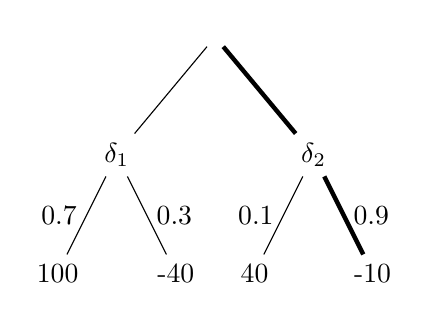
\begin{tikzpicture}
        \node (a){} [sibling distance = 2.5cm]
            child{
                node (b){$\delta_1$}[sibling distance = 1.5cm]
                child{node(c){100} edge from parent node [left] {0.7}}
                child{node(d){-40} edge from parent node [right] {0.3}}
            }
            child{
                node(e){$\delta_2$}[sibling distance = 1.5cm]
                child{node(f){40} edge from parent[solid, thin] node [left] {0.1}}
                child{node(g){-10} edge from parent node [right] {0.9}}
                edge from parent[ultra thick] 
            };
        \end{tikzpicture}
        
        \textit{Loss minimizing agent}
    \end{minipage}
    \caption{Risk neutral agents' decision-making}
    \label{fig:risk-neutral}
\end{figure}

Figure \ref{fig:risk-neutral} shows two agents that are risk neutral. The first agent is gain-maximizing, and the second agent is loss-minimizing. The gain-maximizing agent will always choose $\delta_1$ because it has a higher potential gain of 100. Whereas the loss-minimizing agent will always choose $\delta_2$ because it has a lower potential loss, even though the probability of losing 10 is much higher than the probability of losing 40, the agent will still choose $\delta_2$. Risk neutral agents will always have a linear utility function. This means that the utility of an outcome is proportional to the outcome itself. More rational agents tend to be more sensitive to risk, especially when dealing with high-stakes situations. In general, rational agents show a tendency to avoid high risks when the payoff is insufficient to compensate for them, and they usually prefer an action course with a lower payoff and a higher probability of success. In addition, rational agents sometimes accept to bear small losses in order to avoid situations where there is a low probability of suffering a very large loss. This type of agent is called \textit{Risk Averse}.

\begin{figure}[H]
    \centering
    \begin{minipage}{.5\textwidth}
      \centering
      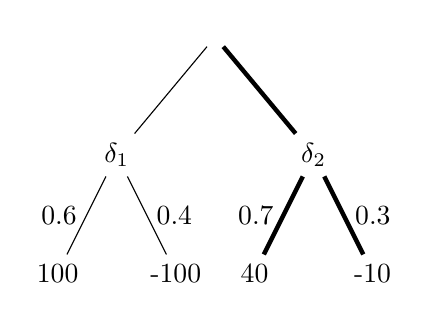
\begin{tikzpicture}
        \node {} [sibling distance = 2.5cm]
            child{
                node{$\delta_1$}[sibling distance = 1.5cm] 
                child{node{100} edge from parent node [left,black] {0.6}}
                child{node{-100} edge from parent node [right] {0.4}}
            }
            child{
                node{$\delta_2$}[sibling distance = 1.5cm]
                child{node{40} edge from parent node [left] {0.7}}
                child{node{-10} edge from parent[ultra thick] node [right] {0.3}}
                edge from parent[ultra thick] 
            };
        \end{tikzpicture}
        
        \textit{Lower potential payoff and loss}
    \end{minipage}%
    \begin{minipage}{.5\textwidth}
      \centering
       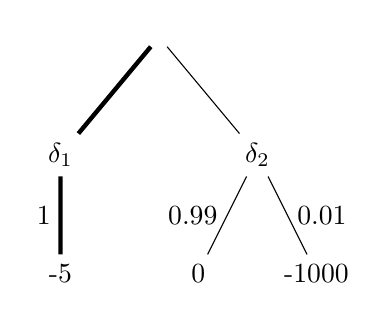
\begin{tikzpicture}
        \node {} [sibling distance = 2.5cm]
            child{
                node{$\delta_1$}[sibling distance = 1.5cm] 
                child{node{-5} edge from parent node [left,black] {1}}
                edge from parent[ultra thick] 
            }
            child{
                node{$\delta_2$}[sibling distance = 1.5cm]
                child{node{0} edge from parent node [left] {0.99}}
                child{node{-1000} edge from parent node [right] {0.01}}
            };
        \end{tikzpicture}
        
        \textit{Small loss over an unlikely very big loss}
    \end{minipage}
    \caption{Risk averse agents' decision-making}
    \label{fig:risk-averse}
\end{figure}

Two distinct situations are shown in Figure \ref{fig:risk-averse} to illustrate how an agent with a risk averse attitude will always choose the action that involves the lowest risk. The utility function of a risk averse agent is concave, with low risk outcomes having a bigger utility score. Some agents are inherently more risk loving (\textit{Risk Seeking}). They will be more willing to take risks in order to achieve a higher payoff, even if it involves a higher risk. The utility function of a risk seeking agent is convex, with high profitability outcomes having a bigger utility score. Figure \ref{fig:risk-seeking} shows how a risk seeking agent will behave in the same previously shown situations.

\begin{figure}[H]
    \centering
    \begin{minipage}{.5\textwidth}
      \centering
      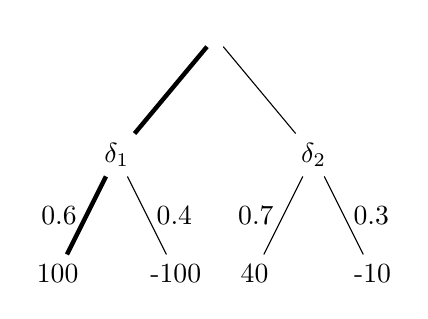
\begin{tikzpicture}
        \node {} [sibling distance = 2.5cm]
            child{
                node{$\delta_1$}[sibling distance = 1.5cm] 
                child{node{100} edge from parent node [left,black] {0.6}}
                child{node{-100} edge from parent[thin] node [right] {0.4}}
                edge from parent[ultra thick] 
            }
            child{
                node{$\delta_2$}[sibling distance = 1.5cm]
                child{node{40} edge from parent node [left] {0.7}}
                child{node{-10} edge from parent node [right] {0.3}}
            };
        \end{tikzpicture}
        
       \textit{Higher potential payoff and loss}
    \end{minipage}%
    \begin{minipage}{.5\textwidth}
      \centering
       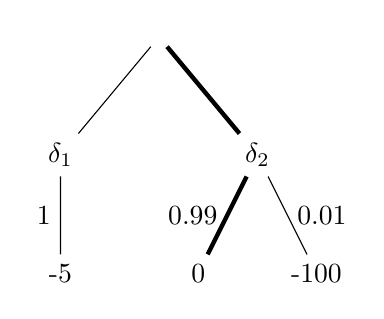
\begin{tikzpicture}
        \node {} [sibling distance = 2.5cm]
            child{
                node{$\delta_1$}[sibling distance = 1.5cm] 
                child{node{-5} edge from parent node [left,black] {1}}
            }
            child{
                node{$\delta_2$}[sibling distance = 1.5cm]
                child{node{0} edge from parent node [left] {0.99}}
                child{node{-100} edge from parent[thin] node [right] {0.01}}
                edge from parent[ultra thick] 
            };
        \end{tikzpicture}
        
         \textit{Accepts the risk}
    \end{minipage}
    \caption{Risk seeking agents' decision-making}
    \label{fig:risk-seeking}
\end{figure}

Typically, the preferences and risk tolerance of an agent will be dynamic, changing based on a broad range of factors such as current wealth, type of risk, and previous experiences. All of these factors make it hard to model the agent's preferences in one mathematical construct; however, \cite{alnazer2022risk} proposes some risk-based utility functions. Figure \ref{fig:risk-based-utility} shows how the utility function of an agent might look based on their risk attitude.




\begin{figure}[H]
    \centering
    \begin{minipage}{.3\textwidth}
      \centering
      \begin{tikzpicture}[scale = 0.5]
        \begin{axis}[
            legend style={at={(1,0.2)},anchor=north east,draw=white},
            axis lines=middle,
            axis line style = thick,
            ticks=none,
            xlabel={Gain},
            ylabel={Utility},
            xlabel style={at={(ticklabel* cs:1)},anchor=north west},
            ylabel style={at={(ticklabel* cs:1)},anchor=north east},
            xmin=0, xmax=10,
            ymin=0, ymax=10,
          ]
          \addplot [
            domain=0:9,
            color=black,
          ]
          {x};
          \addlegendentry{risk neutral}
        \end{axis}
      \end{tikzpicture}
    \end{minipage}
    \hspace{1em}
    \begin{minipage}{.3\textwidth}
      \centering
      \begin{tikzpicture}[scale = 0.5]
        \begin{axis}[
            legend style={at={(1,0.2)},anchor=north east,draw=white},
            axis lines=middle,
            axis line style = thick,
            ticks=none,
            xlabel={Gain},
            ylabel={Utility},
            xlabel style={at={(ticklabel* cs:1)},anchor=north west},
            ylabel style={at={(ticklabel* cs:1)},anchor=north east},
            xmin=0, xmax=100,
            ymin=0, ymax=2,
          ]
  
          \addplot [
            domain=1:80,
            color=black,
            samples=100
          ]
          {log10(x)};
          \addlegendentry{risk averse}
        \end{axis}
      \end{tikzpicture}
    \end{minipage}
    \hspace{1em}
    \begin{minipage}{.3\textwidth}
      \centering
      \begin{tikzpicture}[scale = 0.5]
        \begin{axis}[
            legend style={at={(1,0.2)},anchor=north east,draw=white},
            axis lines=middle,
            axis line style = thick,
            ticks=none,
            xlabel={Gain},
            ylabel={Utility},
            xlabel style={at={(ticklabel* cs:1)},anchor=north west},
            ylabel style={at={(ticklabel* cs:1)},anchor=north east},
            xmin=0, xmax=10,
            ymin=0, ymax=100,
          ]
          \addplot [
            domain=-2:9,
            color=black,
            samples=100
          ]
          {x^2};
          \addlegendentry{risk seeking}
        \end{axis}
      \end{tikzpicture}
    \end{minipage}
    \caption{Different risk-based utility functions}
    \label{fig:risk-based-utility}
\end{figure}

At the end of this section, we would like to point out that although it has been shown \cite{kahneman2013prospect} that the expected utility theory fails as a descriptive theory due to its inability to successfully predict human behavior in some situations, it is a very suitable normative theory that can be used to guide the decision-making process of rational agents, especially when combined with a good dynamic utility function.